\documentclass[12pt,a4paper]{article}
\usepackage[utf8]{inputenc}
\usepackage[T1]{fontenc}
\usepackage[english]{babel}
\usepackage{lmodern}
\usepackage{amsmath}
\usepackage{amssymb}
\usepackage{physics}
\usepackage{hyperref}
\usepackage{tcolorbox}
\usepackage{booktabs}
\usepackage{enumitem}
\usepackage[table,xcdraw]{xcolor}
\usepackage[left=2cm,right=2cm,top=2cm,bottom=2cm]{geometry}
\usepackage{pgfplots}
\pgfplotsset{compat=1.18}
\usepackage{graphicx}
\usepackage{float}
\usepackage{fancyhdr}
\usepackage{siunitx}
\usepackage{tikz}
\usepackage{adjustbox}
\usetikzlibrary{shapes.geometric}

% Custom Commands
\newcommand{\Tfield}{T(x)}
\newcommand{\alphaEM}{\alpha_{\text{EM}}}
\newcommand{\betaT}{\beta_{\text{T}}}
\newcommand{\Mpl}{M_{\text{Pl}}}
\newcommand{\Tzerot}{T_0(\Tfield)}
\newcommand{\e}{\mathrm{e}}
\newcommand{\alphaEMSI}{\alpha_{\text{EM,SI}}}

% Header and Footer Configuration
\pagestyle{fancy}
\fancyhf{}
\fancyhead[L]{Johann Pascher}
\fancyhead[R]{Biological Structures in the Length Scale Hierarchy}
\fancyfoot[C]{\thepage}
\renewcommand{\headrulewidth}{0.4pt}
\renewcommand{\footrulewidth}{0.4pt}

\hypersetup{
	colorlinks=true,
	linkcolor=blue,
	citecolor=blue,
	urlcolor=blue,
	pdftitle={Biological Anomalies within the Quantization of Length Scales in the T0 Model},
	pdfauthor={Johann Pascher},
	pdfsubject={Theoretical Physics},
	pdfkeywords={T0 Model, length scale quantization, biological structures, emergent properties, time-mass duality}
}

\title{Biological Anomalies within the\\Quantization of Length Scales in the T0 Model}
\author{Johann Pascher}
\date{April 12, 2025}

\begin{document}
	
	\maketitle
	
	\begin{abstract}
		This work investigates the unique position of biological structures within the quantized length scale hierarchy identified in the T0 model. While the quantized hierarchy of length scales, spanning from sub-Planckian to cosmological dimensions, exhibits physically stable regions and ``forbidden zones,'' biological structures appear to possess the ability to form stable structures precisely in these forbidden zones. This anomaly is analyzed within the framework of the T0 model with energy as the base unit and interpreted as a potential fundamental property of life. Theoretical explanations are presented, relying on the specific interaction of biological systems with the intrinsic time field \Tfield, and experimental consequences of this hypothesis are discussed.
	\end{abstract}
	
	\section{Introduction: The Anomaly of Biological Structures}
	
	In the first comprehensive work on the ``Systematic Compilation of Natural Units with Energy as the Base Unit'' \cite{pascher_nateinheiten_2025}, the fundamental quantization of length scales was identified as a central result of the T0 model. This quantization manifests in the preferential existence of physical structures in certain discrete size ranges, described by simple powers of dimensionless constants, as well as in the relative absence of stable structures in the ``forbidden zones'' between these preferred regions.
	
	Particularly striking, however, is that biological structures represent a remarkable exception to this pattern. While fundamental physical entities (elementary particles, atoms, stellar and galactic systems) concentrate in the predicted stable length ranges, biological structures seem to preferentially occupy precisely those ``forbidden zones'' that are unfavorable for purely physical structures.
	
	This anomaly, briefly hinted at in the original work, is analyzed in greater detail below, and its potential implications for understanding life within the framework of the T0 model are explored.
	
	\section{Recap of Length Scale Quantization}
	
	For reference: In the T0 model, a quantization of length scales was identified according to the formula:
	
	\begin{equation}
		L_n = l_P \times \prod_{i} (\alpha_i)^{n_i}
	\end{equation}
	
	where:
	\begin{itemize}
		\item $L_n$ represents a preferred length scale
		\item $l_P$ is the Planck length (reference unit)
		\item $\alpha_i$ are fundamental dimensionless constants ($\alphaEM$, $\betaT$, $\xi$)
		\item $n_i$ are integer or rational exponents describing the ``quantum numbers'' of the respective scale
	\end{itemize}
	
	This quantization leads to preferred length ranges where stable physical structures exist, while so-called ``forbidden zones'' lie between these ranges, in which few stable physical structures are found.
	
	\begin{figure}[h]
		\centering
		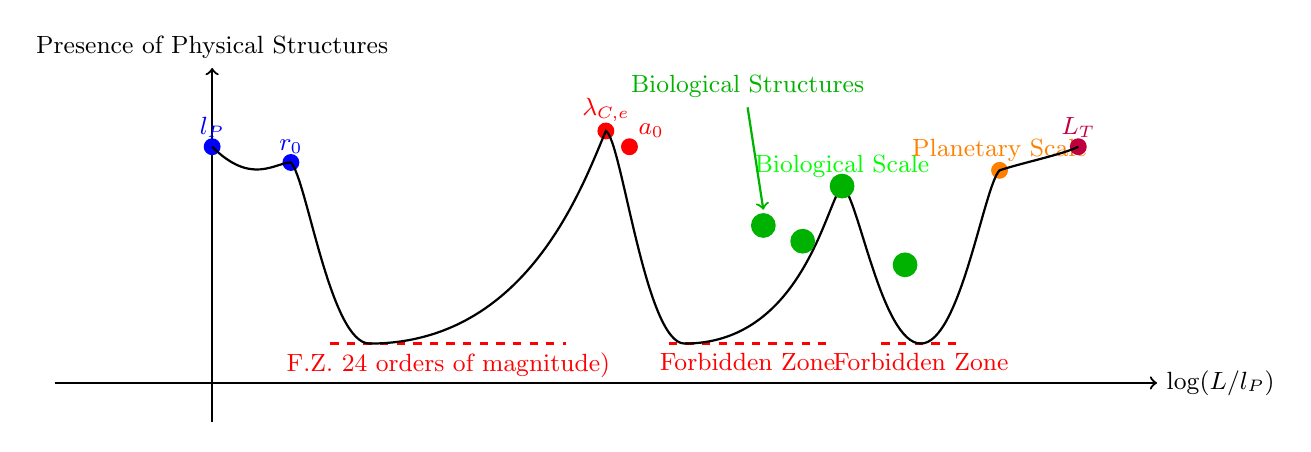
\begin{tikzpicture}
			\small
			\draw[thick,->] (-2,0) -- (12,0) node[right] {$\log(L/l_P)$};
			\draw[thick,->] (0,-0.5) -- (0,4) node[above] {Presence of Physical Structures};
			
			% Important scales
			\filldraw[blue] (0,3) circle (0.1) node[above] {$l_P$};
			\filldraw[blue] (1,2.8) circle (0.1) node[above] {$r_0$};
			\filldraw[red] (5,3.2) circle (0.1) node[above] {$\lambda_{C,e}$};
			\filldraw[red] (5.3,3) circle (0.1) node[above right] {$a_0$};
			\filldraw[green] (8,2.5) circle (0.1) node[above] {Biological Scale};
			\filldraw[orange] (10,2.7) circle (0.1) node[above] {Planetary Scale};
			\filldraw[purple] (11,3) circle (0.1) node[above] {$L_T$};
			
			% Forbidden zones
			\draw[thick, dashed, red] (1.5,0.5) -- (4.5,0.5) node[midway, below] {F.Z. 24 orders of magnitude)};
			\draw[thick, dashed, red] (5.8,0.5) -- (7.8,0.5) node[midway, below] {Forbidden Zone};
			\draw[thick, dashed, red] (8.5,0.5) -- (9.5,0.5) node[midway, below] {Forbidden Zone};
			
			% Stability curve
			\draw[smooth, thick] (0,3) .. controls (0.5,2.5) and (0.8,2.8) .. (1,2.8) 
			.. controls (1.2,2.6) and (1.5,0.5) .. (2,0.5)
			.. controls (4,0.5) and (4.7,2.5) .. (5,3.2)
			.. controls (5.2,3.1) and (5.5,0.5) .. (6,0.5)
			.. controls (7.5,0.5) and (7.8,2.3) .. (8,2.5)
			.. controls (8.2,2.4) and (8.5,0.5) .. (9,0.5)
			.. controls (9.5,0.5) and (9.8,2.5) .. (10,2.7)
			.. controls (10.3,2.8) and (10.8,2.9) .. (11,3);
			
			% Highlight biological structures
			\filldraw[green!70!black] (7,2) circle (0.15);
			\filldraw[green!70!black] (7.5,1.8) circle (0.15);
			\filldraw[green!70!black] (8,2.5) circle (0.15);
			\filldraw[green!70!black] (8.8,1.5) circle (0.15);
			\draw[thick, green!70!black, ->] (6.8,3.5) -- (7,2.2) node[above, green!70!black] at (6.8,3.5) {Biological Structures};
		\end{tikzpicture}
		\caption{Schematic representation of stability centers and forbidden zones along the logarithmic length scale, highlighting biological structures.}
		\label{fig:stability_zones_bio}
	\end{figure}
	
	\section{Position of Biological Structures in the Length Hierarchy}
	
	When considering the characteristic lengths of biological structures:
	
	\begin{table}[h]
		\centering
		\begin{adjustbox}{scale=0.7}
			\begin{tabular}{lllll}
				\hline
				\textbf{Biological Structure} & \textbf{Typical Size} & \textbf{Ratio to $l_P$} & \textbf{Expected Stability Region} & \textbf{Position} \\
				\hline
				DNA Diameter & $\sim 2 \times 10^{-9}$ m & $\sim 10^{-26}$ & Outside & Forbidden Zone \\
				Protein & $\sim 10^{-8}$ m & $\sim 10^{-27}$ & Outside & Forbidden Zone \\
				Bacterium & $\sim 10^{-6}$ m & $\sim 10^{-29}$ & Outside & Forbidden Zone \\
				Typical Cell & $\sim 10^{-5}$ m & $\sim 10^{-30}$ & Outside & Forbidden Zone \\
				Multicellular Organism & $\sim 10^{-3}$ – $10^{0}$ m & $\sim 10^{-32}$ – $10^{-35}$ & Outside & Forbidden Zone \\
				\hline
			\end{tabular}
		\end{adjustbox}
		\caption{Position of biological structures in the length scale hierarchy}
		\label{tab:bio_structures}
	\end{table}
	
	It is clear that virtually all biological structures exist in size ranges that lie between the preferred quantization points of the length scale. The entire spectrum of biological organization—from biomolecules to cells to multicellular organisms—falls within the ``forbidden zones'' of the quantization scheme.
	
	This raises fundamental questions:
	\begin{enumerate}
		\item How can life form stable structures in regions that are theoretically unfavorable for stable physical structures?
		\item Is this anomaly coincidental or fundamental to the nature of life?
		\item What mechanisms enable biological systems to overcome the constraints of length scale quantization?
	\end{enumerate}
	
	\section{Theoretical Explanations within the T0 Model Framework}
	
	Within the context of the T0 model, several theoretical explanations for this biological anomaly can be proposed:
	
	\subsection{Emergence Hypothesis}
	
	Life could be understood as an emergent phenomenon characterized precisely by its ability to create stability in ``forbidden zones.'' The fundamental property of living systems lies in their ability to organize far from thermodynamic equilibrium and form structures that would not be stable under pure equilibrium conditions.
	
	In the T0 model, this can be formalized as:
	
	\begin{equation}
		\nabla^2\Tfield_{\text{bio}} \approx -\frac{\rho}{\Tfield^2} + \delta_{\text{bio}}(\vec{x}, t)
	\end{equation}
	
	where $\delta_{\text{bio}}(\vec{x}, t)$ represents a biological correction term that, through information-driven energy conversion, modifies the local dynamics of the intrinsic time field, thereby enabling stability in otherwise unstable length ranges.
	
	\subsection{Complexity-Mediated Time Field Interaction}
	
	The unique property of biological systems could lie in their specific interaction with the intrinsic time field \Tfield:
	
	\begin{equation}
		\Tfield_{\text{bio}} = \frac{\hbar}{\max(mc^2, \omega)} \cdot \Omega(\text{Complexity})
	\end{equation}
	
	where $\Omega(\text{Complexity})$ is a functional quantifying the information-processing complexity of the system. This approach leads to a modified length scale quantization for biological systems:
	
	\begin{equation}
		L_{\text{bio}} = l_P \times \prod_{i} (\alpha_i)^{n_i} \times \Omega(\text{Complexity})^{1/2}
	\end{equation}
	
	This expression implies that biological systems, through their complexity and information processing, can continuously modulate the otherwise discrete length scale quantization, allowing them to exist even in forbidden zones.
	
	\subsection{Information-Based Decoupling}
	
	A third possibility is that biological systems partially decouple from physical fundamental laws by using information as a fundamental organizational principle. In the T0 model, this could mean that the effective coupling to the time field experienced by biological structures differs from that of purely physical systems:
	
	\begin{equation}
		\betaT^{\text{bio}} = \betaT \cdot f(I/S)
	\end{equation}
	
	where $I$ denotes the information content and $S$ the entropy of the system. Through this modified coupling, biological structures can exist in length ranges that would be unstable for ordinary physical systems.
	
	\section{Experimental Consequences and Testing Opportunities}
	
	The proposed hypotheses lead to experimentally verifiable predictions:
	
	\begin{enumerate}
		\item \textbf{Different Decoherence Rates}: Biological structures should exhibit a reduced quantum decoherence rate compared to non-biological structures of similar size and mass. This could be tested through precision interferometry on biomolecular structures.
		
		\item \textbf{Nonlinear Response to External Time Fields}: Biological systems should respond differently to external time dilation fields (e.g., gravitational gradients) than non-biological systems of similar composition. This could be investigated through precision measurements of biological activity in varying gravitational fields.
		
		\item \textbf{Information-Dependent Stability}: The stability of biological structures should show a stronger correlation with their information content than with their pure physical composition. This could be tested through comparative analyses of biological structures with different information content but similar physical structure.
		
		\item \textbf{Length-Dependent Biological Activity}: Biochemical reactions should exhibit anomalies in their reaction rates that correlate with the predicted length scale quantization. In particular, reactions with characteristic lengths near quantization points should display different kinetic properties than those operating in ``forbidden zones.''
	\end{enumerate}
	
	\section{Philosophical Implications}
	
	The observed anomaly of biological structures in length scale quantization has profound philosophical implications for understanding life in the context of fundamental physical laws:
	
	\begin{enumerate}
		\item \textbf{Life as a Fundamental Phenomenon}: Life may not only be seen as a complex outcome of physical laws but as a fundamental phenomenon operating complementarily to known physical principles.
		
		\item \textbf{Bridge Between Physics and Information}: The ability of biological systems to exist in ``forbidden zones'' may point to a fundamental connection between physical laws and information processing that goes beyond known statistical physics.
		
		\item \textbf{Time Field as a Mediator of Consciousness}: The specific interaction of biological systems with the time field \Tfield could provide a physical basis for the phenomenon of consciousness, often considered irreducible to conventional physical processes.
		
		\item \textbf{Teleological Interpretation}: The positioning of biological structures in forbidden zones may suggest a teleological principle extending beyond pure causal physics—not in the sense of external guidance, but as an emergent property of the T0 model itself.
	\end{enumerate}
	
	\section{Summary and Outlook}
	
	The anomaly of biological structures in the length scale quantization of the T0 model represents a remarkable finding, suggesting a deep connection between the fundamental properties of the universe and the nature of life. The fact that biological structures preferentially occupy precisely those length ranges that are unstable for ordinary physical structures indicates that life may play a fundamental role in the physical cosmos, beyond that of a random assembly of complex molecules.
	
	The T0 model, with energy as the base unit and the setting $\alphaEM = \betaT = 1$, provides a theoretical framework in which this anomaly can not only be described but also explained. Through the specific properties of the intrinsic time field \Tfield and its interaction with information-processing systems, the model opens new perspectives for understanding life as an integral part of fundamental physical reality.
	
	Future research should focus on experimentally verifying the proposed hypotheses, particularly through precision measurements of quantum coherence in biological systems and their response to external time fields. This could lead not only to a deeper understanding of life but also to new insights into the fundamental structure of the universe within the T0 model framework.
	
	\section{Further Anomalies in the Length Scale Hierarchy}
	
	Biological structures are not the only entities positioned outside the preferred length scales. There are other notable physical phenomena exhibiting similar anomalies:
	
	\subsection{Water as an Anomalous Medium}
	
	Water exhibits a variety of anomalies distinguishing it from other liquids:
	
	\begin{itemize}
		\item \textbf{Density Anomaly}: Water reaches its highest density at 4°C, not at the freezing point
		\item \textbf{High Specific Heat Capacity}: Significantly higher than comparable liquids
		\item \textbf{Surface Tension}: Unusually high for such a small molecular structure
		\item \textbf{Hydrogen Bonds}: Form a dynamic network structure
	\end{itemize}
	
	In the context of the T0 model, these anomalies may suggest that water, like biological structures, has a special interaction with the intrinsic time field \Tfield. The characteristic length scale of this interaction is approximately $10^{-10}$ m (distance between water molecules via hydrogen bonds), which also lies in a ``forbidden zone'' of length scale quantization.
	
	Notably, water serves as the basis of life—this shared anomaly may indicate that both phenomena interact with \Tfield through similar mechanisms.
	
	\subsection{Superconductivity and Other Quantum Coherence Phenomena}
	
	Superconductors of various material classes exhibit macroscopic quantum effects at different characteristic length scales:
	
	\begin{table}[h]
		\centering
		\begin{adjustbox}{scale=0.75}
			\begin{tabular}{lllll}
				\hline
				\textbf{Superconductor Type} & \textbf{Coherence Length} & \textbf{Ratio to $l_P$} & \textbf{Position} & \textbf{Feature} \\
				\hline
				Type-I Superconductor (Pb, Hg) & $\sim 10^{-7}$ m & $\sim 10^{-28}$ & Forbidden Zone & Complete Meissner Effect \\
				Type-II Superconductor (Nb$_3$Sn) & $\sim 10^{-8}$ m & $\sim 10^{-27}$ & Forbidden Zone & Flux Tube State \\
				Cuprate HTS (YBCO) & $\sim 10^{-9}$ m & $\sim 10^{-26}$ & Forbidden Zone & High Transition Temperature \\
				Iron Pnictides & $\sim 10^{-9}$ m & $\sim 10^{-26}$ & Forbidden Zone & Unconventional Mechanism \\
				\hline
			\end{tabular}
		\end{adjustbox}
		\caption{Coherence lengths of different superconductor types}
		\label{tab:supercond}
	\end{table}
	
	Superconducting quantum coherence occurs precisely in those length ranges that should be ``forbidden'' according to the quantization theory. This suggests a common mechanism allowing both superconductors and biological structures to overcome the constraints of quantized length scales.
	
	\subsection{Other Anomalous Phenomena in Forbidden Length Ranges}
	
	The list of phenomena preferentially existing in the ``forbidden zones'' of length scale quantization is remarkably extensive and includes further significant examples:
	
	\begin{table}[h]
		\centering
		\begin{adjustbox}{scale=0.65}
			\begin{tabular}{lllll}
				\hline
				\textbf{Phenomenon} & \textbf{Characteristic Length} & \textbf{Ratio to $l_P$} & \textbf{Position} & \textbf{Special Property} \\
				\hline
				Quasicrystals & $\sim 10^{-9}$ - $10^{-8}$ m & $\sim 10^{-26}$ & Forbidden Zone & Ordered but aperiodic structure \\
				Fractals in Nature & Multi-Scale & Spanning & Multiple Zones & Scale-spanning self-similarity \\
				Bose-Einstein Condensates & $\sim 10^{-6}$ m & $\sim 10^{-29}$ & Forbidden Zone & Macroscopic quantum state \\
				Soft Matter & $\sim 10^{-8}$ - $10^{-6}$ m & $\sim 10^{-27}$ & Forbidden Zone & Liquid crystalline order \\
				Cosmic Filaments & $\sim 10^{22}$ - $10^{24}$ m & $\sim 10^{-59}$ & Forbidden Zone & Topological defects in the cosmos \\
				Turbulent Flows & Multi-Scale & Spanning & Multiple Zones & Hierarchy of vortex structures \\
				Ferromagnetic Domains & $\sim 10^{-6}$ - $10^{-4}$ m & $\sim 10^{-29}$ & Forbidden Zone & Spontaneous symmetry breaking \\
				Topological Insulators & $\sim 10^{-8}$ - $10^{-7}$ m & $\sim 10^{-27}$ & Forbidden Zone & Topologically protected edge states \\
				\hline
			\end{tabular}
		\end{adjustbox}
		\caption{Further anomalous phenomena in forbidden length ranges}
		\label{tab:more_anomalies}
	\end{table}
	
	Particularly noteworthy are:
	
	\subsubsection{Quasicrystals and Aperiodic Order}
	
	Quasicrystals exhibit long-range order without periodicity, with forbidden symmetries (e.g., five-fold). These seemingly contradictory properties allow them to exist in a length range that should be unstable according to harmonic length scale quantization. In the T0 model, this could be explained by a specific modulation of the time field induced by aperiodic order.
	
	\subsubsection{Fractal Structures and Scale-Spanning Self-Similarity}
	
	Fractal structures in nature—from coastlines to blood vessel systems to tree structures—show self-similarity across various orders of magnitude. This property allows them to ``bridge'' the discrete preferred length scales and create continuity through forbidden zones. Within the T0 model, the fractal dimension could directly measure the modification of the time field.
	
	\subsubsection{Topologically Protected States}
	
	Topological insulators, certain quantum materials, and cosmic defects exhibit topologically protected states robust against local perturbations. This topological stability could be a fundamental mechanism enabling stable structures in the forbidden zones of length scale quantization.
	
	\subsubsection{Macroscopic Quantum Coherence}
	
	Bose-Einstein condensates and related phenomena demonstrate that macroscopic quantum coherence is possible in regions far from preferred length scales. This suggests a deeper connection between quantum coherence and stability in forbidden zones.
	
	\subsection{Common Stabilization Mechanisms}
	
	The impressive diversity of phenomena preferentially existing in the forbidden zones of length scale quantization suggests the existence of general stabilization mechanisms. In the T0 model, these can be systematized:
	
	\subsubsection{Information-Based Stabilization}
	
	The first mechanism is based on information and complexity:
	
	\begin{itemize}
		\item \textbf{Biological Structures}: Stabilized by genetic and epigenetic information
		\item \textbf{Water}: Stabilized by collective excitations of the hydrogen bond network
		\item \textbf{Superconductors}: Stabilized by coherent many-particle states (Cooper pairs)
		\item \textbf{Quasicrystals}: Stabilized by aperiodic but ordered information
	\end{itemize}
	
	In the T0 model, this can be formalized as a modification of the time field through cooperative effects:
	
	\begin{equation}
		\Tfield_{\text{coop}} = \Tfield \cdot \exp\left(\frac{I_{\text{coop}}}{k_B T}\right)
	\end{equation}
	
	where $I_{\text{coop}}$ represents a measure of the cooperative information of the system.
	
	\subsubsection{Topological Stabilization}
	
	The second mechanism is based on topological properties:
	
	\begin{itemize}
		\item \textbf{Topological Insulators}: Protected by topological invariants
		\item \textbf{Fractal Structures}: Stabilized by scale-spanning self-similarity
		\item \textbf{Cosmic Defects}: Topologically stable configurations
		\item \textbf{Ferromagnetic Domains}: Stabilized by domain wall topology
	\end{itemize}
	
	This can be formalized in the T0 model as:
	
	\begin{equation}
		\Tfield_{\text{topo}} = \Tfield \cdot (1 + \chi \cdot \mathcal{T})
	\end{equation}
	
	where $\mathcal{T}$ represents the topological charge or invariant of the system, and $\chi$ is a coupling constant.
	
	\subsubsection{Dynamic Stabilization}
	
	The third mechanism is based on dynamic, far-from-equilibrium processes:
	
	\begin{itemize}
		\item \textbf{Turbulent Structures}: Stabilized by energy cascades across different scales
		\item \textbf{Biological Homeostasis}: Stabilized by active regulatory mechanisms
		\item \textbf{Soft Matter}: Stabilized by collective dynamics
	\end{itemize}
	
	In the T0 model, this can be formalized as:
	
	\begin{equation}
		\Tfield_{\text{dyn}} = \Tfield \cdot \left(1 + \kappa \cdot \frac{\dot{S}_{\text{prod}}}{S_{\text{eq}}}\right)
	\end{equation}
	
	where $\dot{S}_{\text{prod}}$ represents the entropy production rate and $S_{\text{eq}}$ the equilibrium entropy of the system.
	
	\subsection{Unified Perspective: Ordered Complexity in Forbidden Zones}
	
	The existence of these diverse, seemingly independent anomalies, all sharing the property of existing in the forbidden zones of length scale quantization, points to a deeper principle. In the T0 model, this can be formulated as the ``principle of ordered complexity in forbidden zones'':
	
	\begin{tcolorbox}[colback=blue!5!white,colframe=blue!75!black,title=Principle of Ordered Complexity in Forbidden Zones]
		Systems with a sufficiently high degree of ordered complexity (whether through information, topology, or dynamics) can overcome the destabilizing effects of the intrinsic time field \Tfield in the forbidden zones of length scale quantization and form stable structures there. This stability is mediated by a local modification of the time field, which can be expressed in the general form
		\begin{equation}
			\Tfield_{\text{mod}} = \Tfield \cdot F(\Omega)
		\end{equation}
		where $\Omega$ represents an appropriate measure of ordered complexity.
	\end{tcolorbox}
	
	This principle offers a unifying perspective on the various anomalous phenomena and explains why the most complex and information-rich structures in the universe—from biological organisms to water to exotic quantum materials—preferentially exist in those length ranges that are ``forbidden'' for ordinary physical structures.
	
	The strong evidence from so many different fields of physics provides compelling support for the T0 model and suggests fundamental connections between quantum coherence, information, topology, and biological organization, all mediated by the intrinsic time field \Tfield.
	
	\section{Experimental Precision Measurement Methods for Model Verification}
	
	To empirically verify the proposed stabilization mechanisms for structures in forbidden zones, high-precision measurement methods tailored to the different phenomenon classes are required:
	
	\subsection{High-Resolution Measurement of Time Field Modulations}
	
	The T0 model predicts that systems forming stable structures in forbidden length ranges locally modulate the intrinsic time field \Tfield. This modulation should be experimentally detectable through:
	
	\begin{enumerate}
		\item \textbf{Interferometric Methods}: Quantum interferometers could be used to detect subtle phase differences arising from local time field modulation. In particular, biological samples should exhibit a characteristic interference signature stemming from their information-based stabilization.
		
		\item \textbf{Time-Resolved Spectroscopy}: Ultrafast spectroscopy in the femto- to attosecond range could be used to measure the dynamic modulation of the time field by living systems. The hypothesis predicts that time resolution near biological structures should deviate from standard quantum behavior.
		
		\item \textbf{Precision Gravimetry}: Since the time field \Tfield in the T0 model is linked to the gravitational field, high-precision gravitational measurements near structures in forbidden zones should reveal subtle anomalies consistent with the model.
	\end{enumerate}
	
	\subsection{Comparative Measurements at Forbidden/Permitted Interfaces}
	
	Particularly informative would be measurements on systems exhibiting structures in both permitted and forbidden length ranges simultaneously:
	
	\begin{itemize}
		\item \textbf{Biological-Inorganic Hybrid Structures}: Biomineralizations such as bones or mollusk shells, where biological structures directly interface with crystalline structures, provide a natural test system. The T0 model predicts that a measurable gradient in the time field structure should occur at such interfaces.
		
		\item \textbf{Quasicrystal-Crystal Transitions}: Materials exhibiting transitions between periodic crystals (in permitted zones) and quasicrystals (in forbidden zones) should show corresponding transition signatures in the time field.
	\end{itemize}
	
	A promising experimental setup would involve placing quantum sensors near such interfaces to measure local variations in the effective action of the time field.
	
	\section{Formal Description of Stabilization Mechanisms}
	
	The three identified stabilization mechanisms—information-based, topological, and dynamic—can be formalized more precisely within the T0 model framework. Below, we develop a unified mathematical framework integrating these mechanisms.
	
	\subsection{Generalized Time Field Modification}
	
	We begin with a generalized ansatz function for the modification of the intrinsic time field:
	
	\begin{equation}
		\Tfield_{\text{mod}} = \Tfield_0 \cdot \left[ 1 + \sum_i \lambda_i \cdot \Phi_i(\mathbf{x}, t) \right]
	\end{equation}
	
	where $\Tfield_0$ is the unmodified time field, $\lambda_i$ are coupling constants, and $\Phi_i(\mathbf{x}, t)$ are modulation functions corresponding to the different stabilization mechanisms.
	
	\subsection{Functional Form of Modulation Functions}
	
	For each of the three stabilization mechanisms, a specific functional form can be derived:
	
	\subsubsection{Information-Based Modulation}
	
	\begin{equation}
		\Phi_{\text{info}}(\mathbf{x}, t) = \exp\left(\frac{I(\mathbf{x}, t)}{k_B T}\right) - 1
	\end{equation}
	
	where $I(\mathbf{x}, t)$ represents the local information density. This can be specified for different systems:
	
	\begin{itemize}
		\item For biological systems: $I_{\text{bio}} = I_{\text{gen}} + I_{\text{epigen}} + I_{\text{metab}}$
		\item For water: $I_{\text{H2O}} = I_{\text{H-Bond-Network}}$
		\item For superconductors: $I_{\text{SC}} = I_{\text{Cooper-Pairs}}$
	\end{itemize}
	
	\subsubsection{Topological Modulation}
	
	\begin{equation}
		\Phi_{\text{topo}}(\mathbf{x}, t) = \chi \cdot \mathcal{T}(\mathbf{x}, t)
	\end{equation}
	
	where $\mathcal{T}(\mathbf{x}, t)$ represents an appropriate topological invariant:
	
	\begin{itemize}
		\item For topological insulators: Chern number or Z2 invariant
		\item For fractal structures: Hausdorff dimension minus Euclidean dimension
		\item For cosmic defects: Winding number or Brouwer degree
	\end{itemize}
	
	\subsubsection{Dynamic Modulation}
	
	\begin{equation}
		\Phi_{\text{dyn}}(\mathbf{x}, t) = \kappa \cdot \frac{\dot{S}_{\text{prod}}(\mathbf{x}, t)}{S_{\text{eq}}}
	\end{equation}
	
	where $\dot{S}_{\text{prod}}(\mathbf{x}, t)$ represents the local entropy production rate and $S_{\text{eq}}$ the equilibrium entropy.
	
	\subsection{Field Equations with Modified Time Field}
	
	With the modified time field, corresponding adjusted field equations arise in the T0 model:
	
	\begin{equation}
		\nabla^2\Tfield_{\text{mod}} \approx -\frac{\rho}{\Tfield_{\text{mod}}^2} + \sum_i \nabla \cdot \left( \lambda_i \nabla \Phi_i \right)
	\end{equation}
	
	This equation describes how stable structures in forbidden zones are enabled through local modifications of the time field. The solutions to this equation should precisely reproduce the observed length scales of the anomalous phenomena.
	
	\section{Phase Transitions Between Permitted and Forbidden Zones}
	
	A particularly insightful aspect of the T0 model is the prediction of specific phase transitions occurring when systems switch between permitted and forbidden length ranges. These transitions should exhibit characteristic signatures that are experimentally detectable.
	
	\subsection{Classification of Transitions}
	
	Within the T0 model framework, different types of transitions can be classified:
	
	\begin{table}[h]
		\centering
		\begin{adjustbox}{scale=0.6}
			\begin{tabular}{lllll}
				\hline
				\textbf{Transition Type} & \textbf{Characteristic} & \textbf{Example System} & \textbf{Order} & \textbf{Time Field Signature} \\
				\hline
				Continuous Transition & Gradual Change & Growing Crystals & Second Order & Gradual Modulation \\
				Discontinuous Transition & Abrupt Change & Phase Transitions in Superconductors & First Order & Abrupt Modulation \\
				Hybrid Transition & Mixed Characteristic & Biomineralization & Mixed & Complex Modulation \\
				Topological Transition & Change in Topological Invariants & Quantum Phase Transitions & – & Topological Defects \\
				\hline
			\end{tabular}
		\end{adjustbox}
		\caption{Classification of transitions between permitted and forbidden length scales}
		\label{tab:transitions}
	\end{table}
	
	\subsection{Emergent Phenomena at Transition Points}
	
	At the transitions between permitted and forbidden zones, the T0 model predicts the occurrence of emergent phenomena:
	
	\begin{enumerate}
		\item \textbf{Increased Fluctuations}: Enhanced quantum fluctuations should occur at transition points, associated with a local ``blurring'' of the time field structure.
		
		\item \textbf{Anomalous Diffusion}: Diffusion processes should exhibit non-Fickian characteristics at transitions, with anomalous exponents directly calculable from the time field modulation functions.
		
		\item \textbf{Coherence Phenomena}: Spontaneous coherence formation should preferentially occur at transitions between permitted and forbidden zones, as the time field is particularly sensitive to information-based stabilization here.
	\end{enumerate}
	
	Particularly interesting is the hypothesis that biological evolution preferentially operates at such transition points, as the flexibility to form new structure types is maximized here while sufficient stability is maintained.
	
	\subsection{Experimental Signatures}
	
	The transitions should be experimentally detectable through the following signatures:
	
	\begin{itemize}
		\item \textbf{Anomalous Heat Capacity}: Systems at the transition should exhibit peaks or discontinuities in heat capacity.
		
		\item \textbf{Altered Relaxation Times}: Characteristic relaxation times should show anomalous scaling behavior at transitions.
		
		\item \textbf{Increased Susceptibility}: The response to external fields should be enhanced at transitions.
	\end{itemize}
	
	These predictions offer concrete experimental tests for the T0 model and its explanation of the stability of structures in forbidden zones.
	
	\section{Implications for Artificial Systems and Technological Applications}
	
	The realization that certain systems can occupy the ``forbidden zones'' of length scale quantization through specific stabilization mechanisms opens fascinating perspectives for technological applications and the development of artificial systems with novel properties.
	
	\subsection{Design of Stable Structures in Forbidden Length Ranges}
	
	Based on the identified stabilization mechanisms, design principles for artificial systems can be derived to deliberately occupy forbidden length ranges:
	
	\begin{enumerate}
		\item \textbf{Information-Based Materials}: Artificial structures with high information density, such as DNA origami, programmable materials, or molecular machines, could be designed to be stable in forbidden zones. This could lead to materials with entirely novel properties.
		
		\item \textbf{Topologically Protected Quantum Technologies}: By leveraging topological stabilization, robust quantum computers could be developed that operate in length ranges theoretically unstable but stabilized through time field modulation.
		
		\item \textbf{Dynamically Stabilized Nanostructures}: Far-from-equilibrium, active nanosystems could utilize dynamic stabilization to exist in forbidden length ranges and perform novel functions there.
	\end{enumerate}
	
	\subsection{Bionics and Biomimetic Approaches}
	
	The unique ability of biological systems to exist in forbidden zones suggests biomimetic approaches:
	
	\begin{itemize}
		\item \textbf{Time Field Modulator Materials}: Modeled after biological systems, materials could be developed that locally modulate the time field, exhibiting properties such as enhanced stability, self-repair, or adaptive response.
		
		\item \textbf{Hierarchical Information Storage}: The multiscale organization of biological information (from DNA to epigenetic regulation to neural networks) could serve as a model for novel information storage and processing systems operating across various length scales.
	\end{itemize}
	
	\subsection{Potential Applications}
	
	The practical utilization of the identified stabilization mechanisms could lead to revolutionary applications:
	
	\begin{table}[h]
		\centering
		\begin{adjustbox}{scale=0.65}
			\begin{tabular}{lll}
				\hline
				\textbf{Application Area} & \textbf{Potential Technology} & \textbf{Underlying Mechanism} \\
				\hline
				Quantum Information Technology & Time field-modulated qubits & Information-based stabilization \\
				Medical Implants & Biomimetic materials with improved interface properties & Hybrid stabilization \\
				Energy Storage & Superconducting storage with elevated transition temperatures & Topological stabilization \\
				Catalysis & Quasicrystalline catalysts with enhanced efficiency & Information-based stabilization \\
				Sensing & High-sensitivity quantum sensors in forbidden length ranges & Dynamic stabilization \\
				Communication Technology & Time field-modulated signal transmission & Information-based stabilization \\
				\hline
			\end{tabular}
		\end{adjustbox}
		\caption{Potential technological applications based on stabilization mechanisms in forbidden zones}
		\label{tab:applications}
	\end{table}
	
	These applications are not merely theoretical possibilities but could represent concrete pathways to overcoming current technological limitations by leveraging the fundamental properties of the time field and its modification.
	
	\bibliographystyle{apsrev4-2}
	\begin{thebibliography}{99}
		\bibitem{pascher_nateinheiten_2025} J. Pascher, \textit{Systematic Compilation of Natural Units with Energy as the Base Unit}, April 2025.
		\bibitem{pascher_zeit_2025} J. Pascher, \href{https://github.com/jpascher/T0-Time-Mass-Duality/tree/main/2/pdf/English/ZeitEmergentQMEn.pdf}{Time as an Emergent Property in Quantum Mechanics: A Connection Between Relativity, Fine-Structure Constant, and Quantum Dynamics}, March 2025.
		\bibitem{pascher_alpha_2025} J. Pascher, \href{https://github.com/jpascher/T0-Time-Mass-Duality/tree/main/2/pdf/English/NatEinheitenAlpha1En.pdf}{Energy as a Fundamental Unit: Natural Units with $\alphaEM = 1$ in the T0 Model}, March 2025.
		\bibitem{pascher_emergente_2025} J. Pascher, \href{https://github.com/jpascher/T0-Time-Mass-Duality/tree/main/2/pdf/English/EmergentGravT0En.pdf}{Emergent Gravitation in the T0 Model: A Comprehensive Derivation}, April 2025.
		\bibitem{pascher_alphabeta_2025} J. Pascher, \href{https://github.com/jpascher/T0-Time-Mass-Duality/tree/main/2/pdf/English/Alpha1Beta1KonsistenzEn.pdf}{Unified Unit System in the T0 Model: The Consistency of $\alpha = 1$ and $\beta = 1$}, April 2025.
		\bibitem{pascher_perspective_2025} J. Pascher, \href{https://github.com/jpascher/T0-Time-Mass-Duality/tree/main/2/pdf/English/ZeitRaumPascherEn.pdf}{A New Perspective on Time and Space: Johann Pascher’s Revolutionary Ideas}, March 2025.
		\bibitem{pascher_bio_2025} J. Pascher, \textit{Biological Structures as a Manifestation of Time-Mass Duality}, in preparation, April 2025.
	\end{thebibliography}
	
\end{document}